\documentclass[tikz]{standalone}
\usepackage{tikz,amsmath}
\usetikzlibrary{calc}
\tikzstyle{vertex} = [draw, shape=circle, minimum width=.3cm, inner sep=.5pt]
\begin{document}
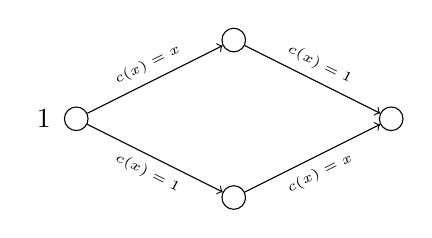
\begin{tikzpicture}[sloped]
    \draw (-1,0) node[vertex] (s) {};
    \draw (1,1) node[vertex] (a) {};
    \draw (1,-1) node[vertex] (b) {};
    \draw (3,0) node[vertex] (t) {};
    \draw [->] (s) -- node [above] {\tiny{$c(x)=x$}} node [below,red] {} (a);
    \draw [->] (s) -- node [below] {\tiny{$c(x)=1$}} node [above,red] {} (b);
    \draw [->] (a) -- node [above] {\tiny{$c(x)=1$}} node [below,red] {} (t);
    \draw [->] (b) -- node [below] {\tiny{$c(x)=x$}} node [above,red] {} (t);
    \node at (s) [left=.2cm] {$\tiny{1}$};
\end{tikzpicture}
\end{document}
